\documentclass{beamer}
%\mode<presentation>
\usepackage[utf8]{inputenc}
\usepackage[english]{babel}
\usetheme{CambridgeUS}
\usecolortheme{dolphin}
\usepackage{amsmath,amssymb,amsfonts, bm}
\usepackage{mathpazo}
\usepackage{graphicx,tabularx,epsfig}
\usepackage[compatibility=false]{caption}
\usepackage{subcaption}
\usepackage{rotating}
\usepackage{mathtools}


\setbeamertemplate{background}{\tikz[overlay,remember picture]\node[opacity=0.07]at (current page.center){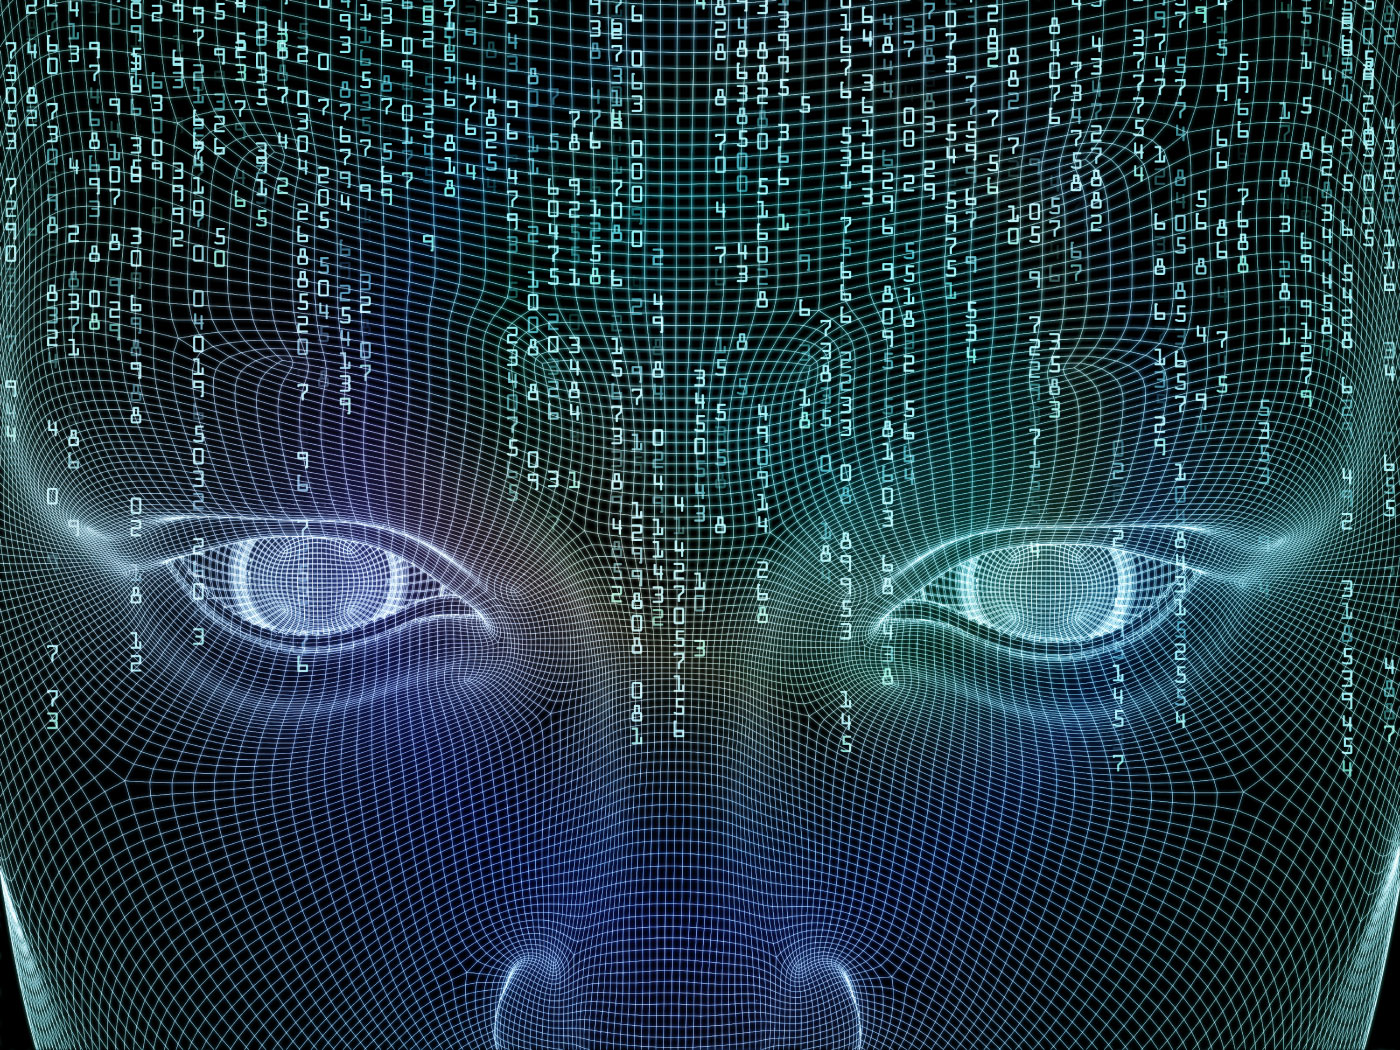
\includegraphics[width=\paperwidth]{pic/bkg}};}
\usepackage{tikz}

\DeclareGraphicsExtensions{.pdf,.png,.jpg,.svg}


\setbeamertemplate{itemize items}[square]
\setbeamertemplate{enumerate items}[square]

\definecolor{Red}{RGB}{190,0,0}
\definecolor{Blue}{RGB}{0,0,190}
\setbeamertemplate{headline}{}



\title[HBT]{Three particle Bose-Einstein correlation}
\author[Attila Bagoly]{Attila Bagoly\\ Eötvös Loránd University \vspace{0.5cm}}
\date[2016.10.20.]{2016.10.20}
\institute[ELTE]{
\large{Supervisor: Máté Csanád}
}

\begin{document}

\begin{frame}
  \titlepage
\end{frame}

\begin{frame}
\frametitle{Contents}
\tableofcontents
\end{frame}


\section{Motivation}
\begin{frame}
\frametitle{Motivation}
\begin{itemize}
\setlength{\itemsep}{12pt}
\item What does $\lambda_2$ mean?
\item Core-Halo: 
	\begin{align}
		\lambda_2=f_C^2\nonumber\\
		\lambda_3 = 2f_C^3+3f_C^2
	\end{align}
\item Partial coherence: 
	\begin{align}
		\lambda_2=f_C^2\big[(1-p_c)^2+2p_c(1-p_c)\big]\nonumber\\
		\lambda_3=2f_C^3\big[(1-p_c)^3+3p_c(1-p_c)^2\big]+3f_C^2\big[(1-p_c)^2+2p_c(1-p_c)\big]
	\end{align}
\item Or other effects: 
	\begin{align}
		\lambda_2 = f_C^2(...)\nonumber\\
		\lambda_3 = 2f_C^3(...)+3f_C^2(...)
	\end{align}
\end{itemize}
\end{frame}

\section{Definitions}
\begin{frame}
\frametitle{Definitions}
\begin{itemize}
\setlength{\itemsep}{12pt}
\item We want to obtain new information about sQGP by measuring 3 particle BE
\item Definition of correlation function:
\begin{equation}
C_3(\bm{k_1}, \bm{k_2}, \bm{k_3})=\frac{N_3(\bm{k_1}, \bm{k_2}, \bm{k_3})}{N_1(\bm{k_1})N_1(\bm{k_2})N_1(\bm{k_3})} \label{eq:e1}
\end{equation}
\item Transverse momentum:
\begin{equation}
p_T=\big|\bm{p}_{T1}+\bm{p}_{T2}+\bm{p}_{T3}\big|/3
\end{equation}
\item Momentum differences: $\bm{k_{ij}}=\bm{k_i}-\bm{k_j}$
\item So we want to measure $C_3(\bm{k_{12}}, \bm{k_{13}}, \bm{k_{23}})$ for different $p_T$ bins
\end{itemize}
\end{frame}


\begin{frame}
\frametitle{Correlation function}
\begin{itemize}
\setlength{\itemsep}{20pt}
\item We use side-out-longitudinal decomposition 
\item Coordinate system: LCMS (longitudinal co-moving system) of the triplet
\item Instead of $\bm{k_{ij}^{\mathrm{LCMS}}}$ we measure correlation as function of 
\begin{equation*}
k_{ij}=|\bm{k_{ij}^{\mathrm{LCMS3}}}|
\end{equation*}
\item Reason: not enough statistics, $q_\mathrm{inv}$ not good as we seen in PPG194
\item $q=\sqrt{k_{12}^2+k_{13}^2+k_{23}^2}$ also not a good choice: no spherical symmetry
\end{itemize}
\end{frame}

\section{What and how we measure}
\begin{frame}
\frametitle{Details of measurement}
\begin{itemize}
\setlength{\itemsep}{22pt}
\item PPG194 generalized to three particle
\item Event-mixing method to measure correlation
\item Momentum difference distributions of pion pairs within the triplet from same event: $A(k_{12}, k_{13}, k_{23})$
\item Background distribution (triplets from different events): $B(k_{12}, k_{13}, k_{23})$
\item Same global, track and pair cuts as PPG194
\end{itemize}
\end{frame}

\begin{frame}
\frametitle{Details of measurement}
\begin{itemize}
\setlength{\itemsep}{16pt}
\item Low bin behavior:
\begin{equation}
k_{ij}\rightarrow 0 \;\;\xRightarrow{\;\;\;?\;\;\;\;}\;\; A,B\rightarrow 0
\end{equation}
\begin{figure}
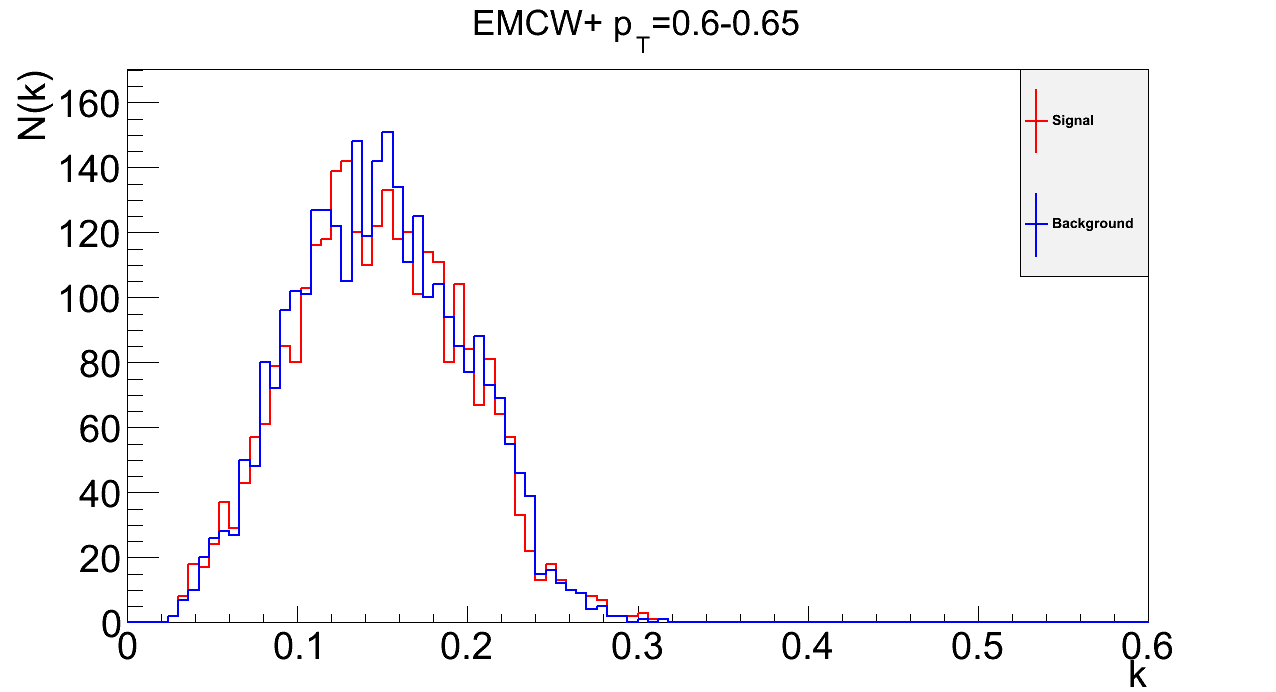
\includegraphics[scale=0.25]{pic/AB}
\end{figure}
\end{itemize}
\end{frame}

\begin{frame}
\frametitle{Details of measurement}
\begin{itemize}
\setlength{\itemsep}{16pt}
\item The correlation:
\begin{equation}
C_3(k_{12}, k_{13}, k_{23})=\frac{A(k_{12}, k_{13}, k_{23})}{B(k_{12}, k_{13}, k_{23})}\frac{\int B}{\int A}
\end{equation}
\item Triangle inequality for $\vec{k}_{12}$, $\vec{k}_{13}$, $\vec{k}_{23}$
\begin{figure}
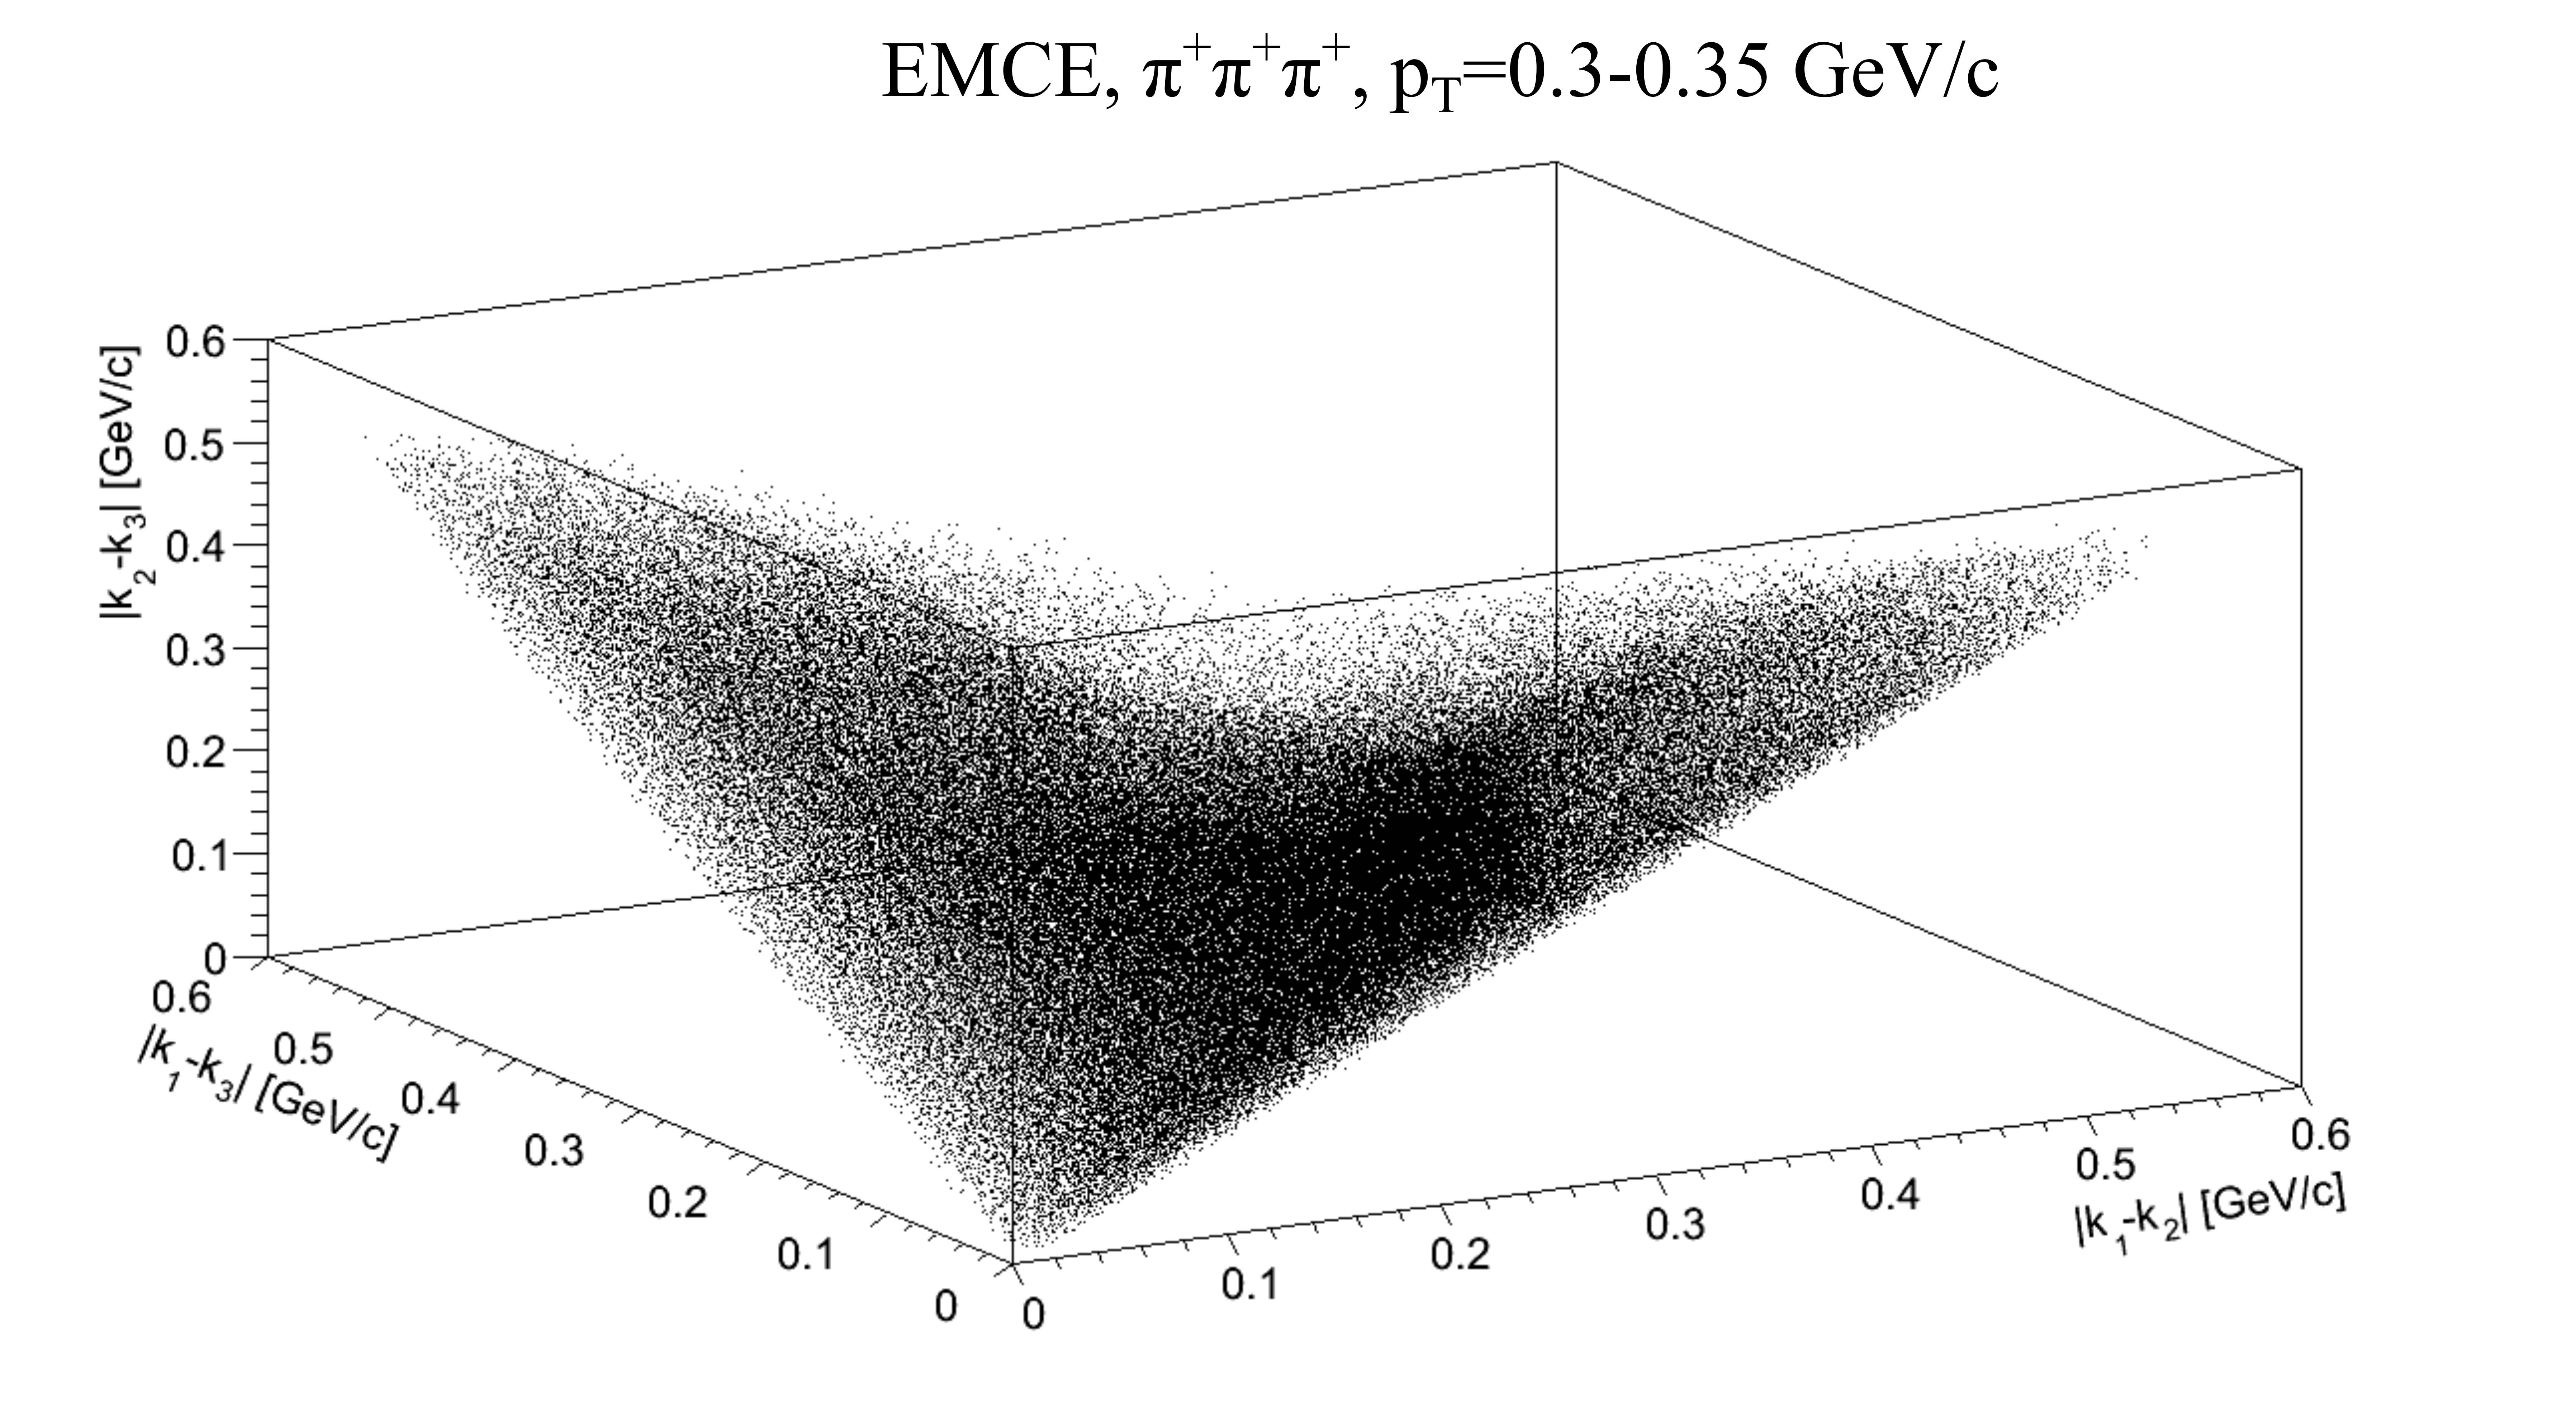
\includegraphics[scale=0.25]{pic/C1}
\end{figure}
\end{itemize}
\end{frame}

\begin{frame}
\frametitle{Details of measurement}
\begin{itemize}
\setlength{\itemsep}{16pt}
\item Order within triplet doesn't matter
\item But when we measure do matter $\Rightarrow$ we have to fold the histogram
		\;\;\;A(5,6,7)\;+=\;A(6,7,5)+A(7,5,6)+A(5,7,6)+A(7,6,5)+A(6,5,7)
\begin{figure}
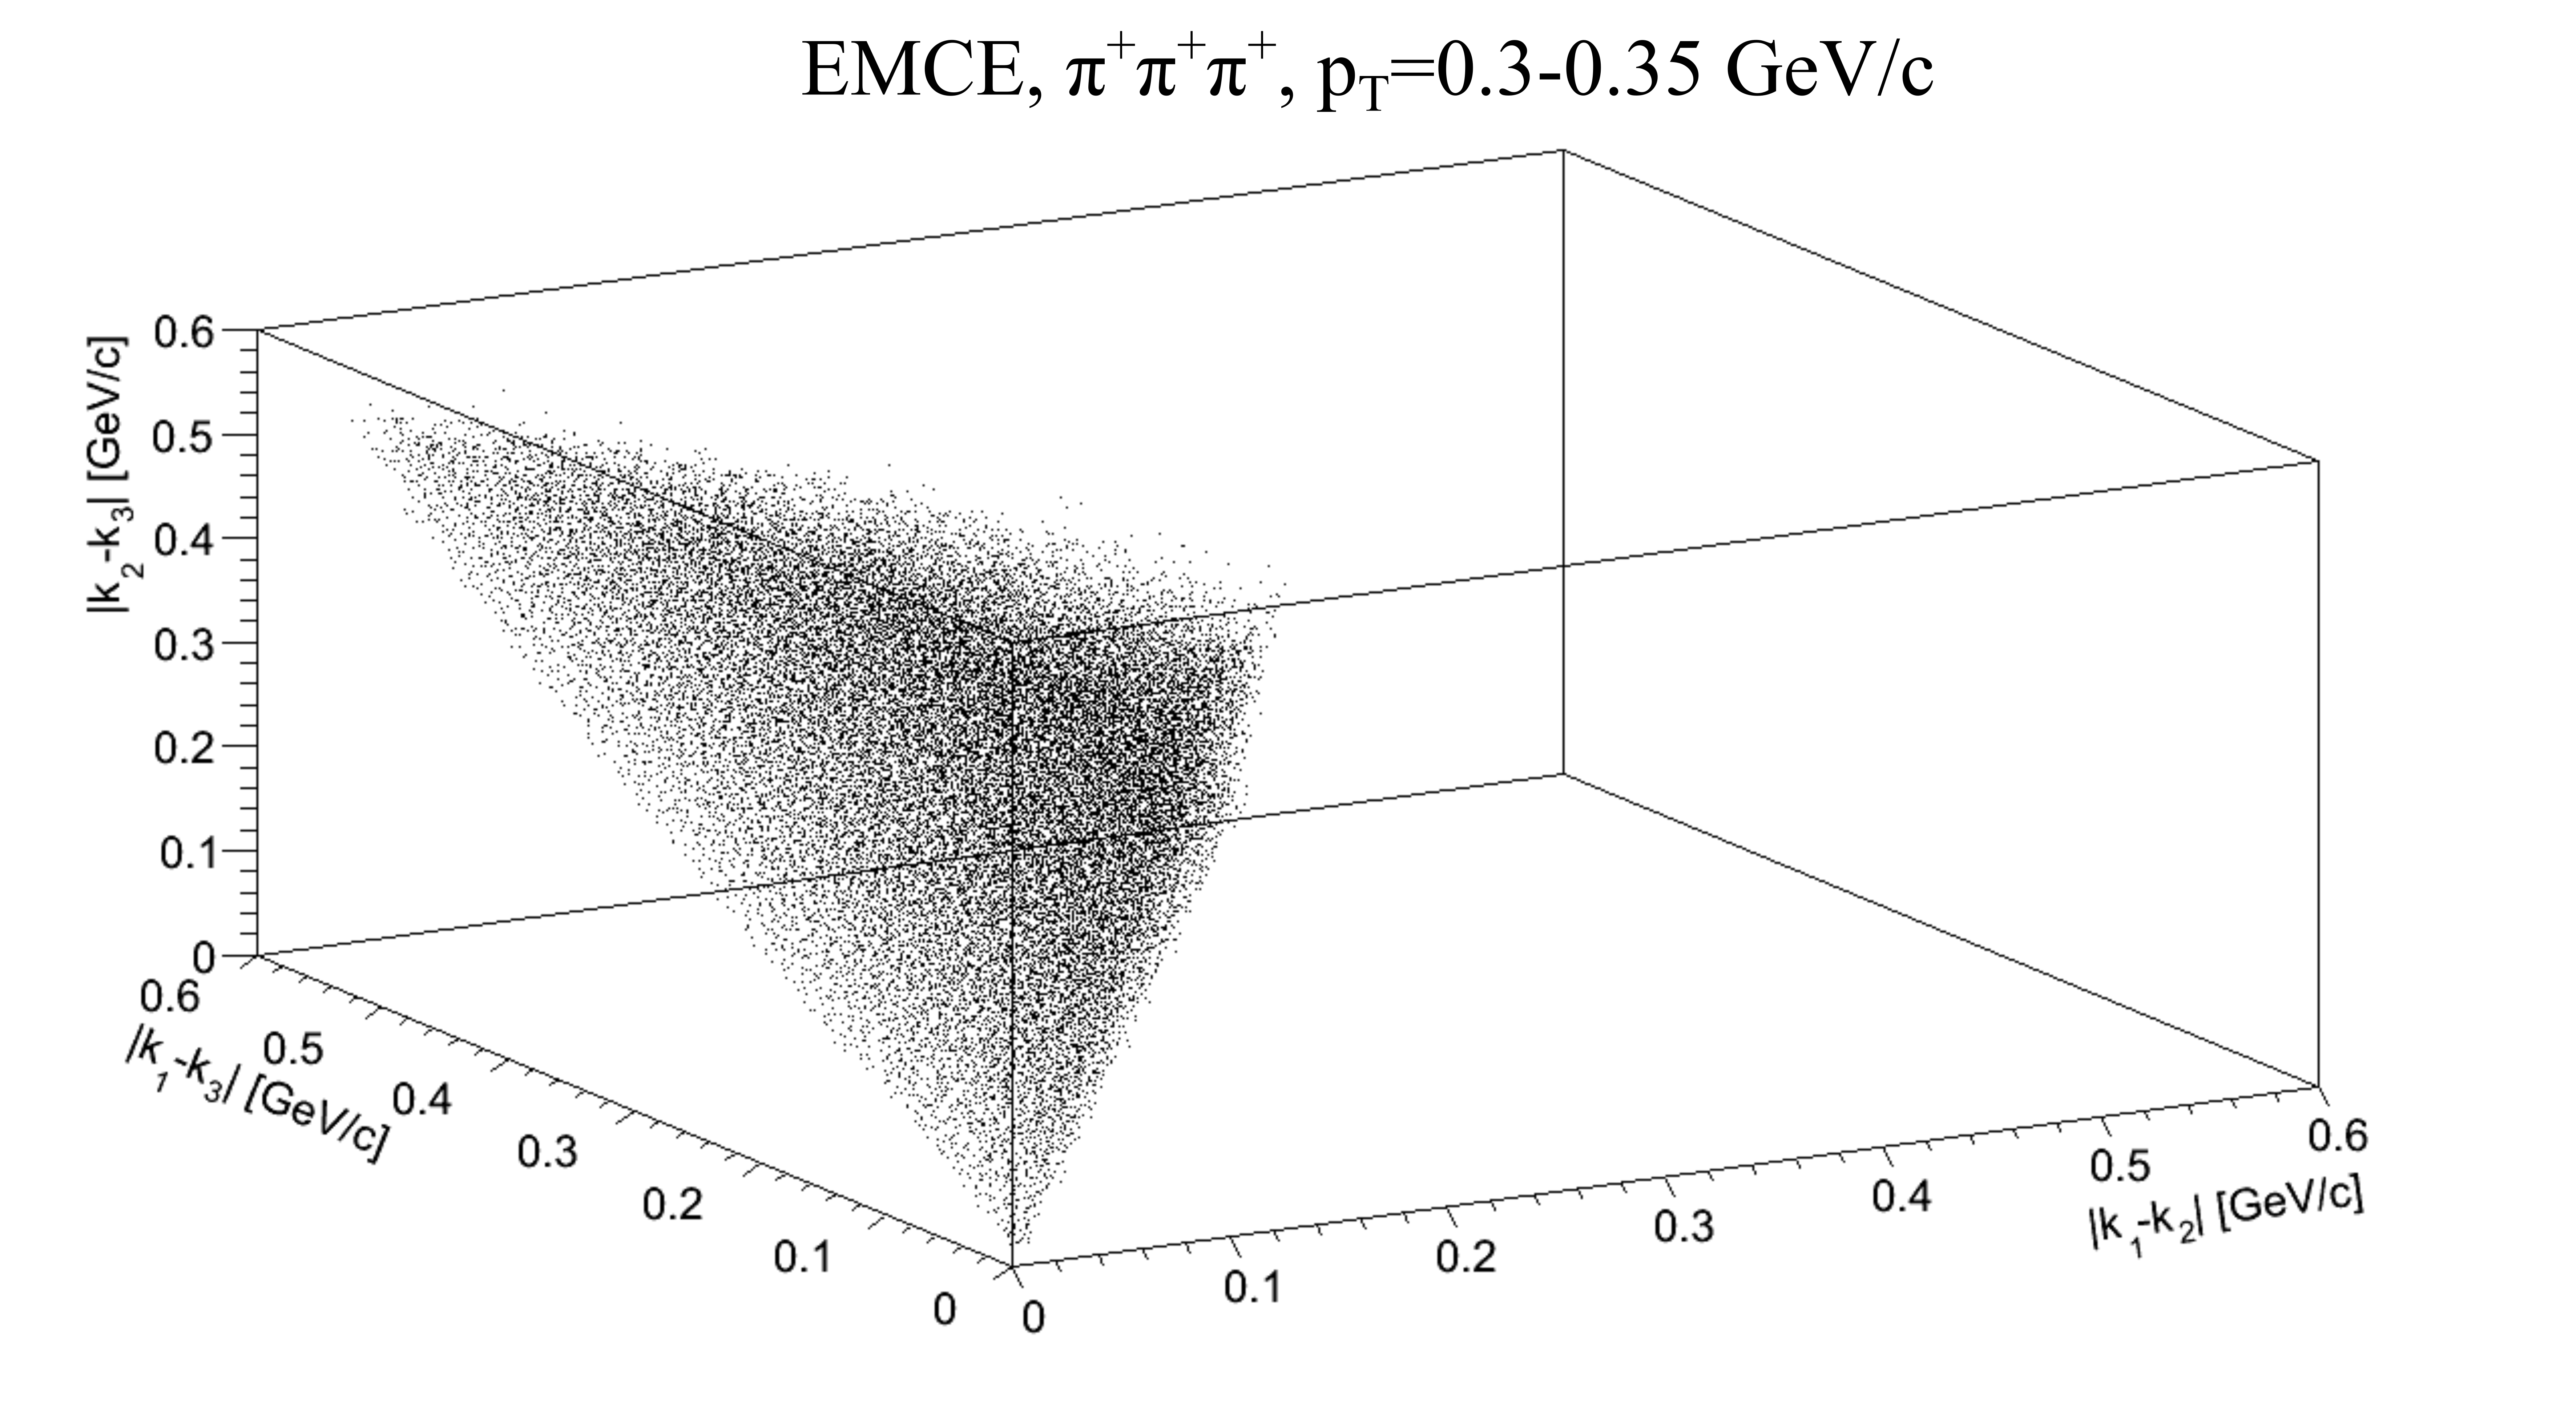
\includegraphics[scale=0.25]{pic/C2}
\end{figure}
\end{itemize}
\end{frame}

\section{Model}
\begin{frame}
\frametitle{Model without Coulomb correction}
\begin{itemize}
\setlength{\itemsep}{16pt}
\item Assumption for source: Levy-distribution
\item Approximation for $C_3$ can be derived ($\mathcal{L}=2f_C^3$):
\begin{align}
C_3^{(0)}(k_{12}, k_{13}, k_{23}) = 1+ \mathcal{L}e^{-0.5(|2k_{12}R_C|^\alpha+|2k_{13}R_C|^\alpha+|2k_{23}R_C|^\alpha)}\nonumber\\
+f_C^2\bigg(e^{|2k_{12}R_C|^\alpha}+e^{|2k_{13}R_C|^\alpha}+e^{|2k_{23}R_C|^\alpha}\bigg)
\end{align}
\item Idea: $\mathcal{L}$ new fitting parameter
\item We already know (from PPG194): $R_C$, $f_C, \alpha$
\item We are looking for: $\lambda_3=\mathcal{L}+3f_C^2$
\end{itemize}
\end{frame}

\begin{frame}
\frametitle{Coulomb correction}
\begin{itemize}
\setlength{\itemsep}{16pt}
\item Corrected model:
\begin{equation}
C_3(k_{12}, k_{13}, k_{23}) = C_3^{(0)}(k_{12}, k_{13}, k_{23})\cdot K_3(k_{12}, k_{13}, k_{23})
\end{equation}
\item ''Generalized Riverside'' method for 3 particle Coulomb problem
\begin{equation}
K_3(k_{12}, k_{13}, k_{23}) \approx K_1(k_{12})K_1(k_{13})K_1(k_{23})
\end{equation}
\end{itemize}
\begin{figure}
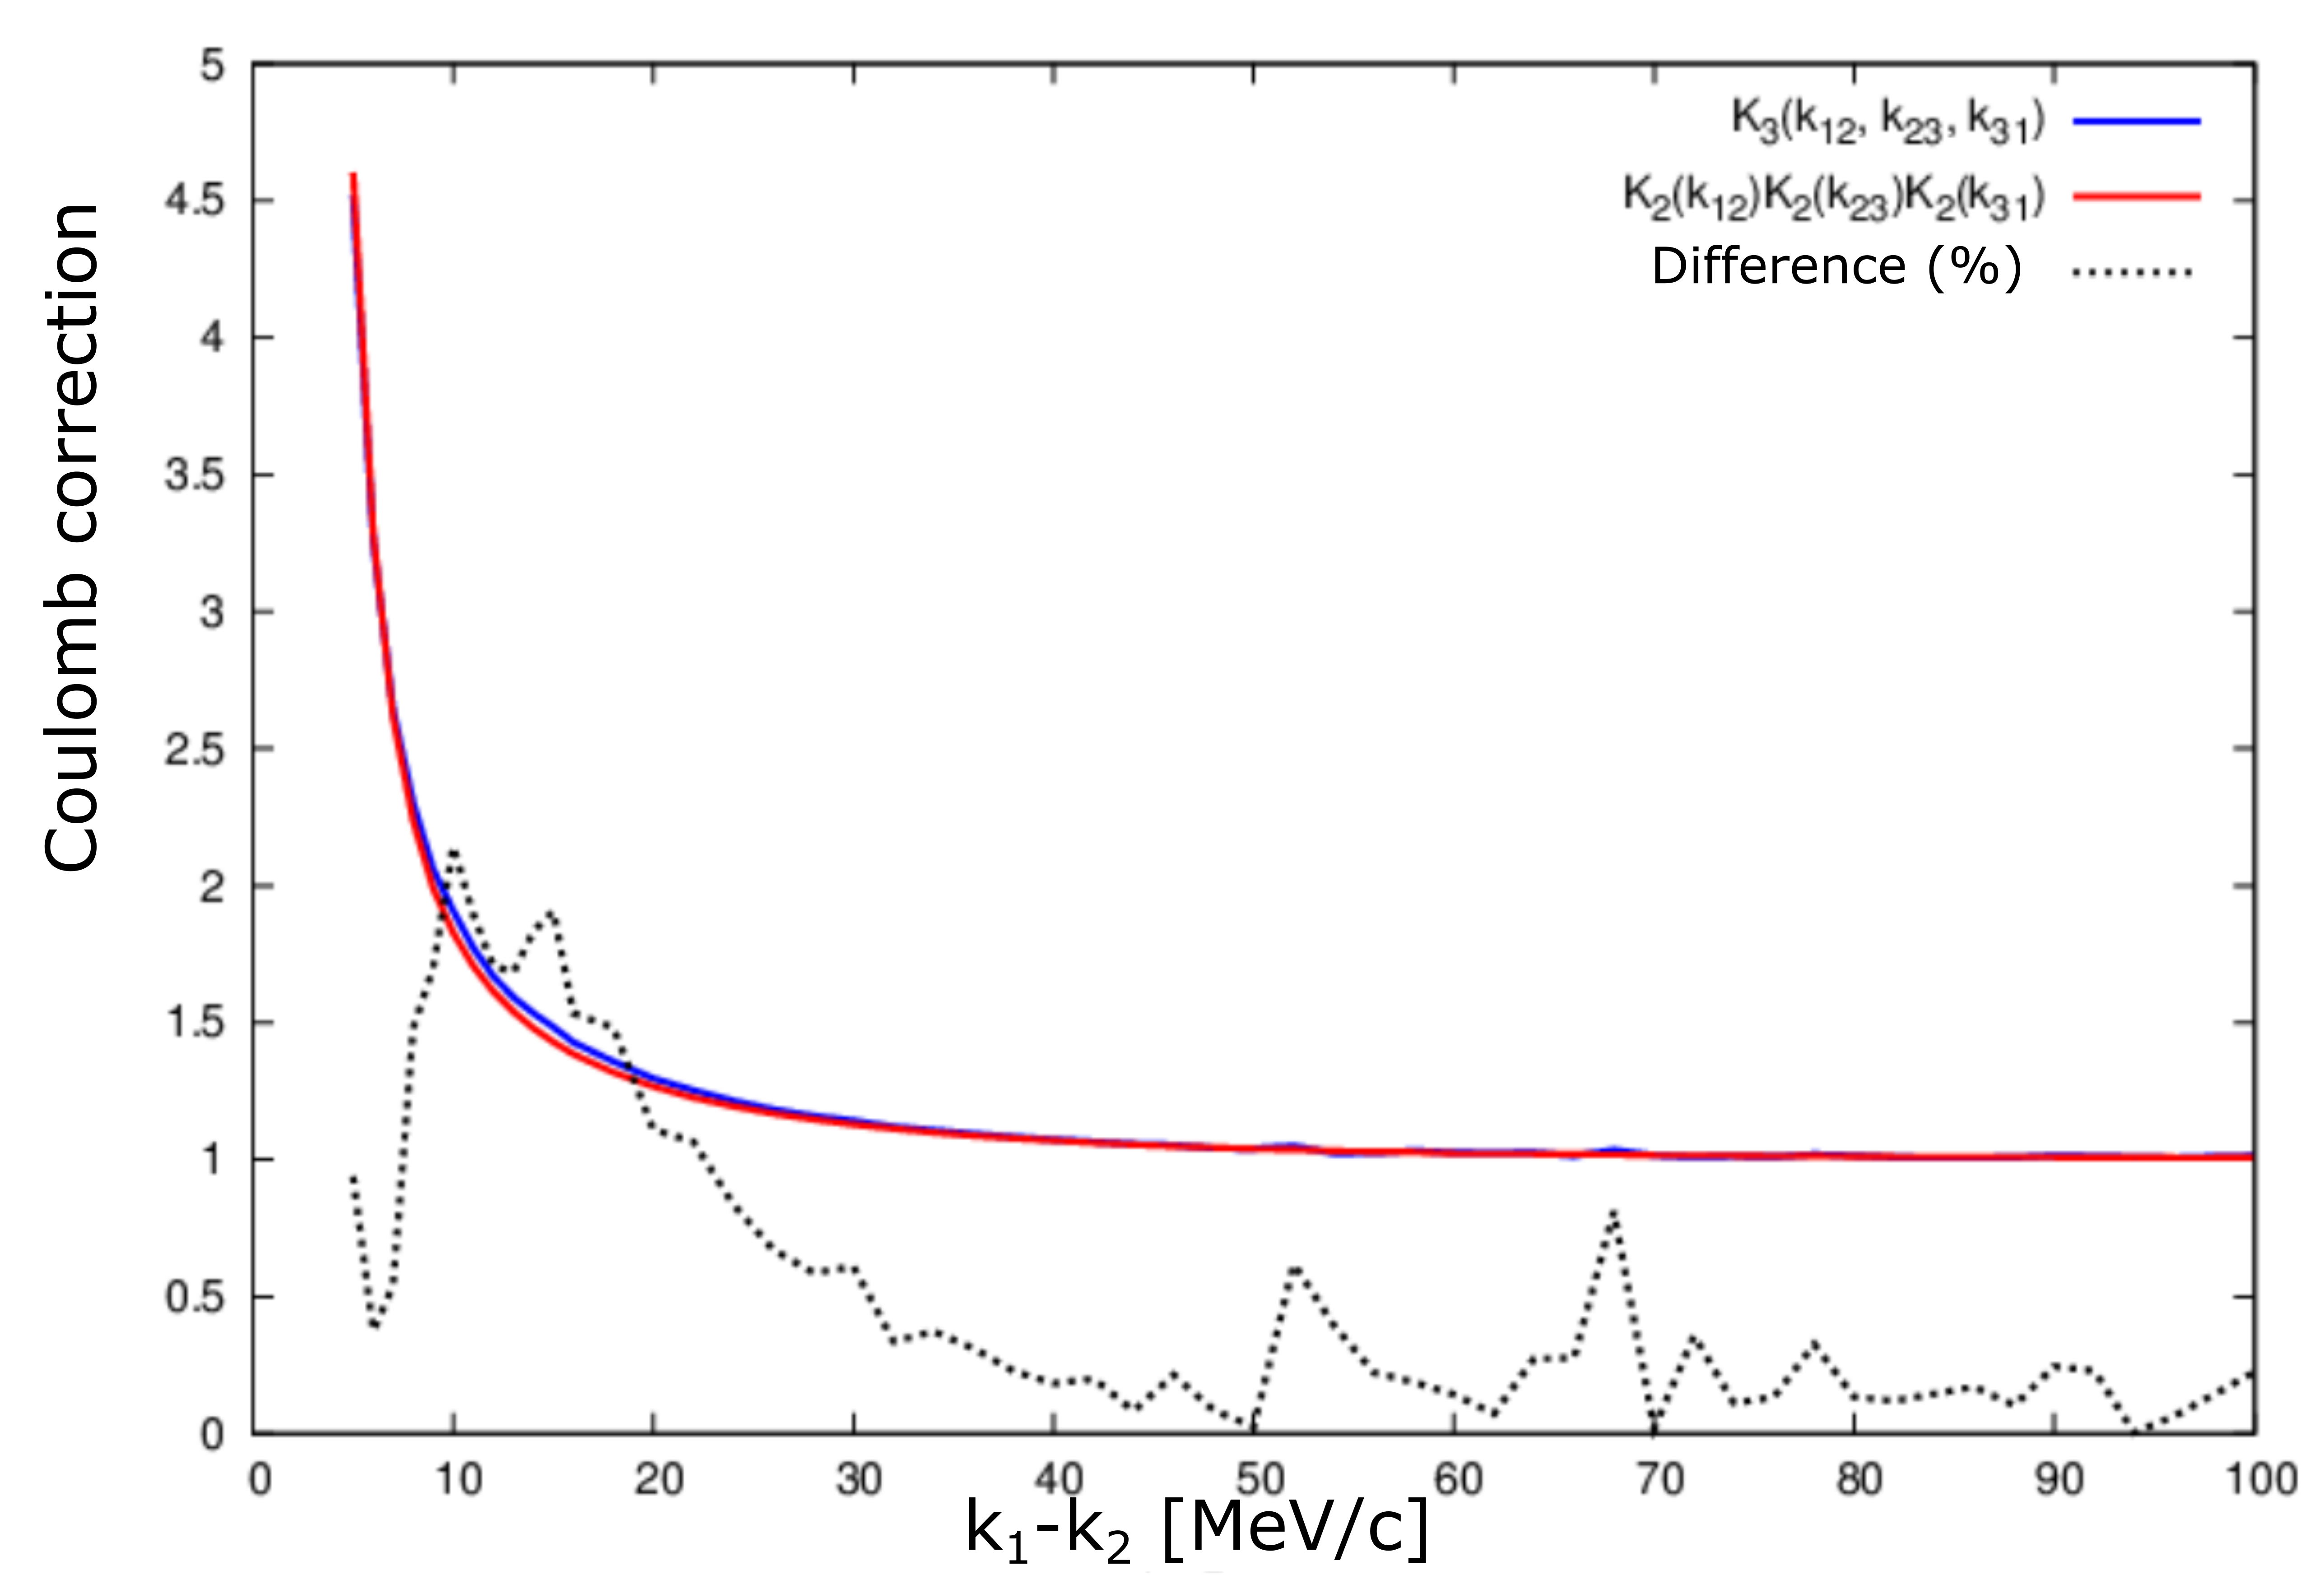
\includegraphics[scale=0.25]{pic/coulomb1}
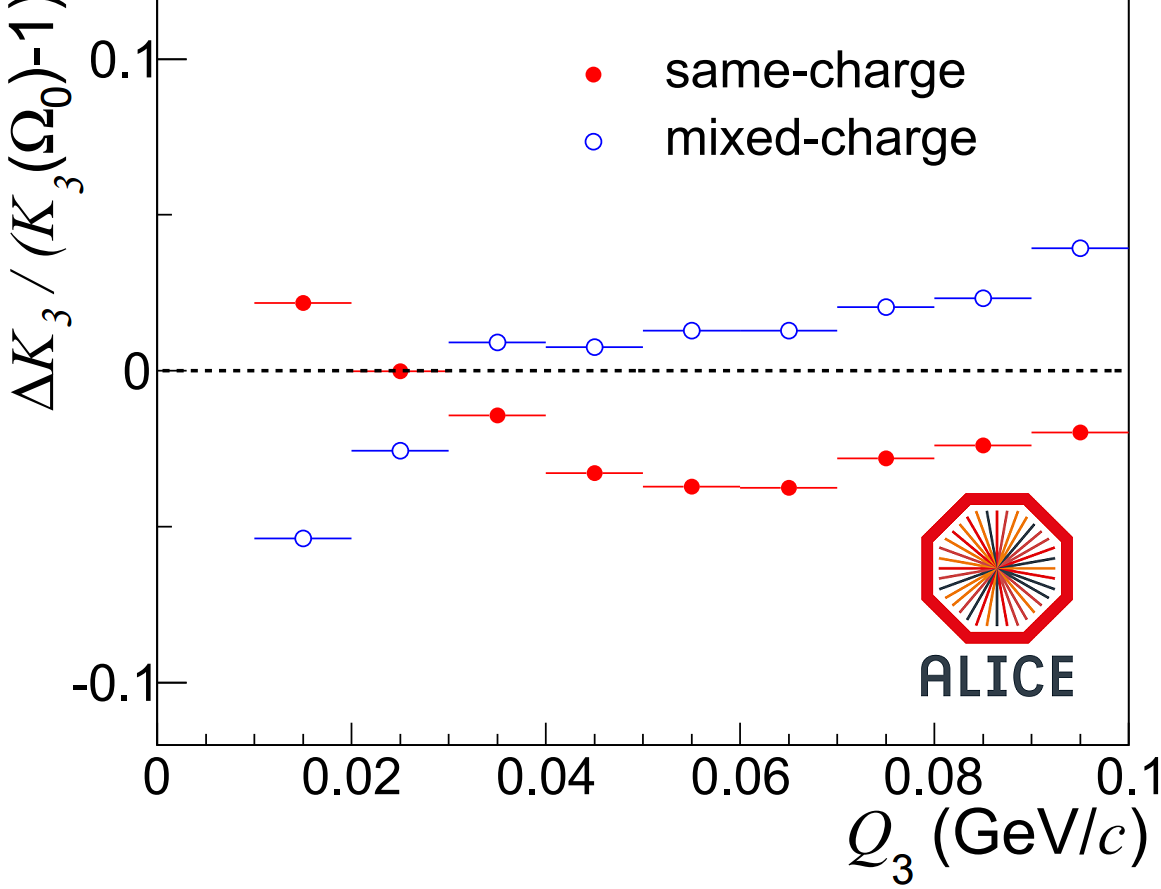
\includegraphics[scale=0.235]{pic/coulomb2}
\end{figure}
\end{frame}

\section{Analysis status}

\begin{frame}
\frametitle{Analysis status}
\begin{itemize}
\item Fittings not quite good: $R, \alpha, f_C$ fixed, $\mathcal{L}$ fitting parameter
\end{itemize}
\begin{figure}
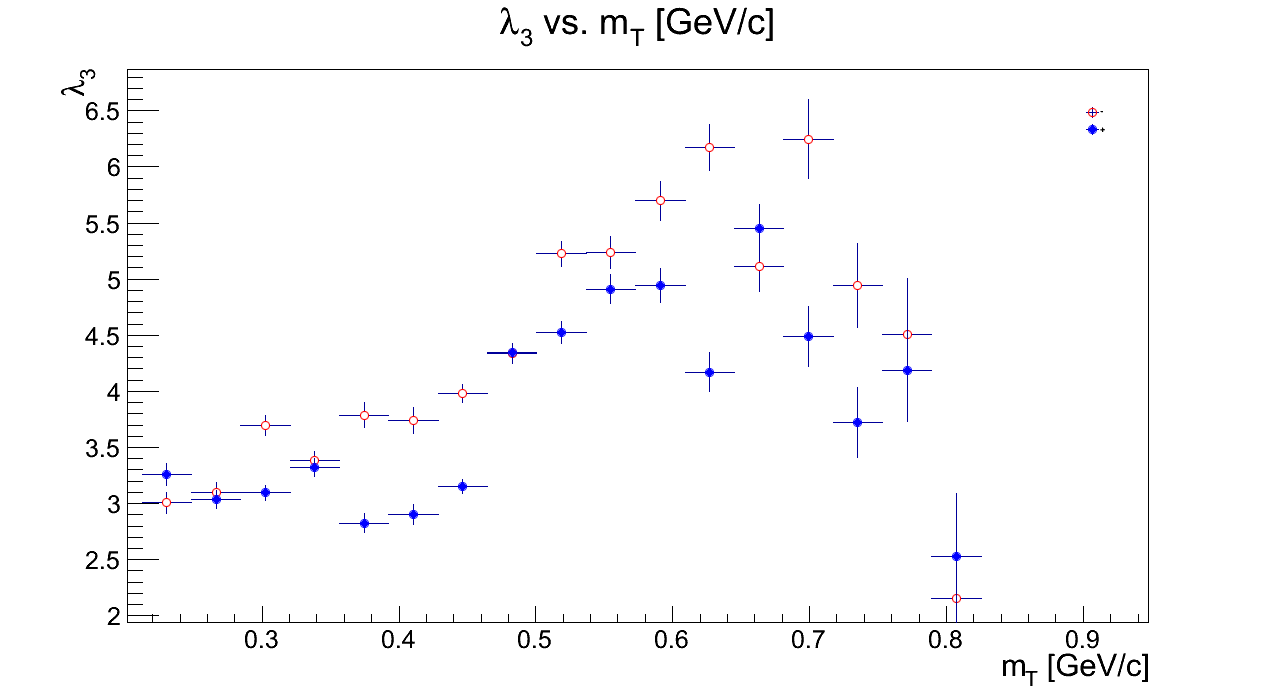
\includegraphics[scale=0.27]{pic/l3}
\end{figure}
\end{frame}

\begin{frame}
\frametitle{Analysis status}
\begin{itemize}
\item Core-Halo transformed out: $\frac{\lambda_3-3\lambda_2}{2\sqrt{\lambda_2^3}}$ not depend on $f_C$
\end{itemize}
\begin{figure}
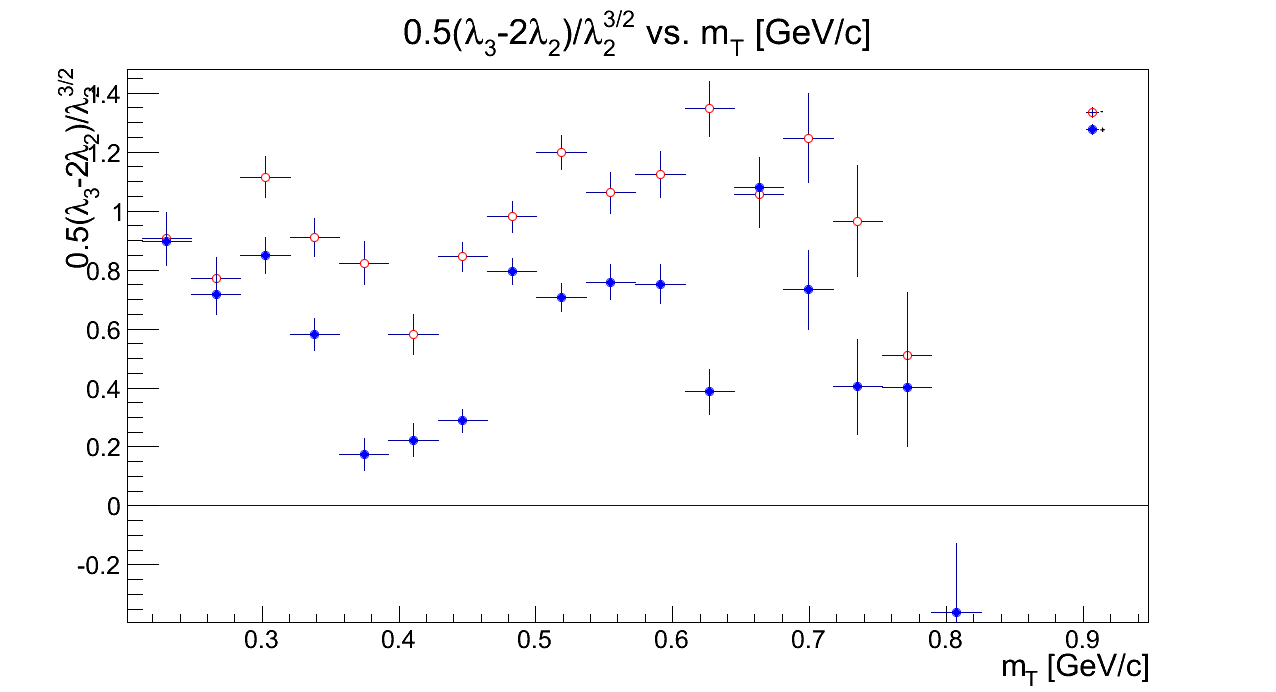
\includegraphics[scale=0.25]{pic/l4}
\end{figure}
\end{frame}





\end{document}

